\section{Introduction}\label{sec:introduction}
% no \IEEEPARstart

Animals utilize tails in a variety of ways: to propel themselves through water; to help improve locomotion and balance; and some even use their tails for hanging on branches or for grasping trees. Balance control while running and hopping, or while gliding and climbing are just few examples of how a tail can help animals to realize robust locomotion \cite{Thomas:Nature2012}. The use of a tail for dynamic stabilization has been reported in the case of dinosaurs, lizards, cats, primates and even humans \cite{ostrom1969osteology,PijnappelsSringer,Walker199841,JusufiIOP2010}. One of the challenges in the design of biologically inspired robot systems is studying phenomena in natural systems and extracting basic knowledge for building similar technical systems. This does not mean only mimicking the nature, but also searching for innovative solutions. One such challenge is to add a tail mechanism to a walking robot so that it improves robot locomotion in a similar way as an animal's tail would do. 
 
A tail can balance the robot's body in both static and dynamic sense. The main technique of using a tail as a dynamic stabilizer for quadruped robot locomotion is to apply additional forces/torques on its body. Uniroo \cite{zeglin1991uniroo} is one of the first robots which uses a single degree of freedom active tail to maintain constant body pitch with the purpose of emulating a hopping kangaroo. Another active tail stabilization case presented in \cite{conf/iros/Chang-SiuLTF11} uses a tail on a wheeled car as a means for robust maneuvering on uneven terrain and stable pitch control by applying the principle of conservation of the momentum. The MIT Cheetah robot \cite{DBLP:conf/iros/BriggsLHK12} uses a tail to improve robot's running capabilities and perform runs up to 30 mph. Additionally, the authors analyze several other artificial mechanisms which can be used for exerting non-contact forces/torques like a reaction wheel, reaction mass, thrusters etc. In \cite{PullinICRA12}, Pullin et all compared the use of a tail to classical differential drive steering for different surface conditions on a crawling mobile robot OctoRoACH. They showed how a tail could be used when rapid turning or evasive maneuvers are required under low friction surface conditions. Learning from aerial robots, one can apply the techniques used in \cite{Korpela2013ICRA,Orsag2012JINT} to model the dynamics of inertial appendages and the impact they have on the underlying robot body. This paper however, wishes to address an alternative use for a tail, its static balancing capabilities. A tail is envisioned here as a counterweight capable of shifting its center of mass so as to balance effectively the robot body.
 
\begin{figure}
                \centering
                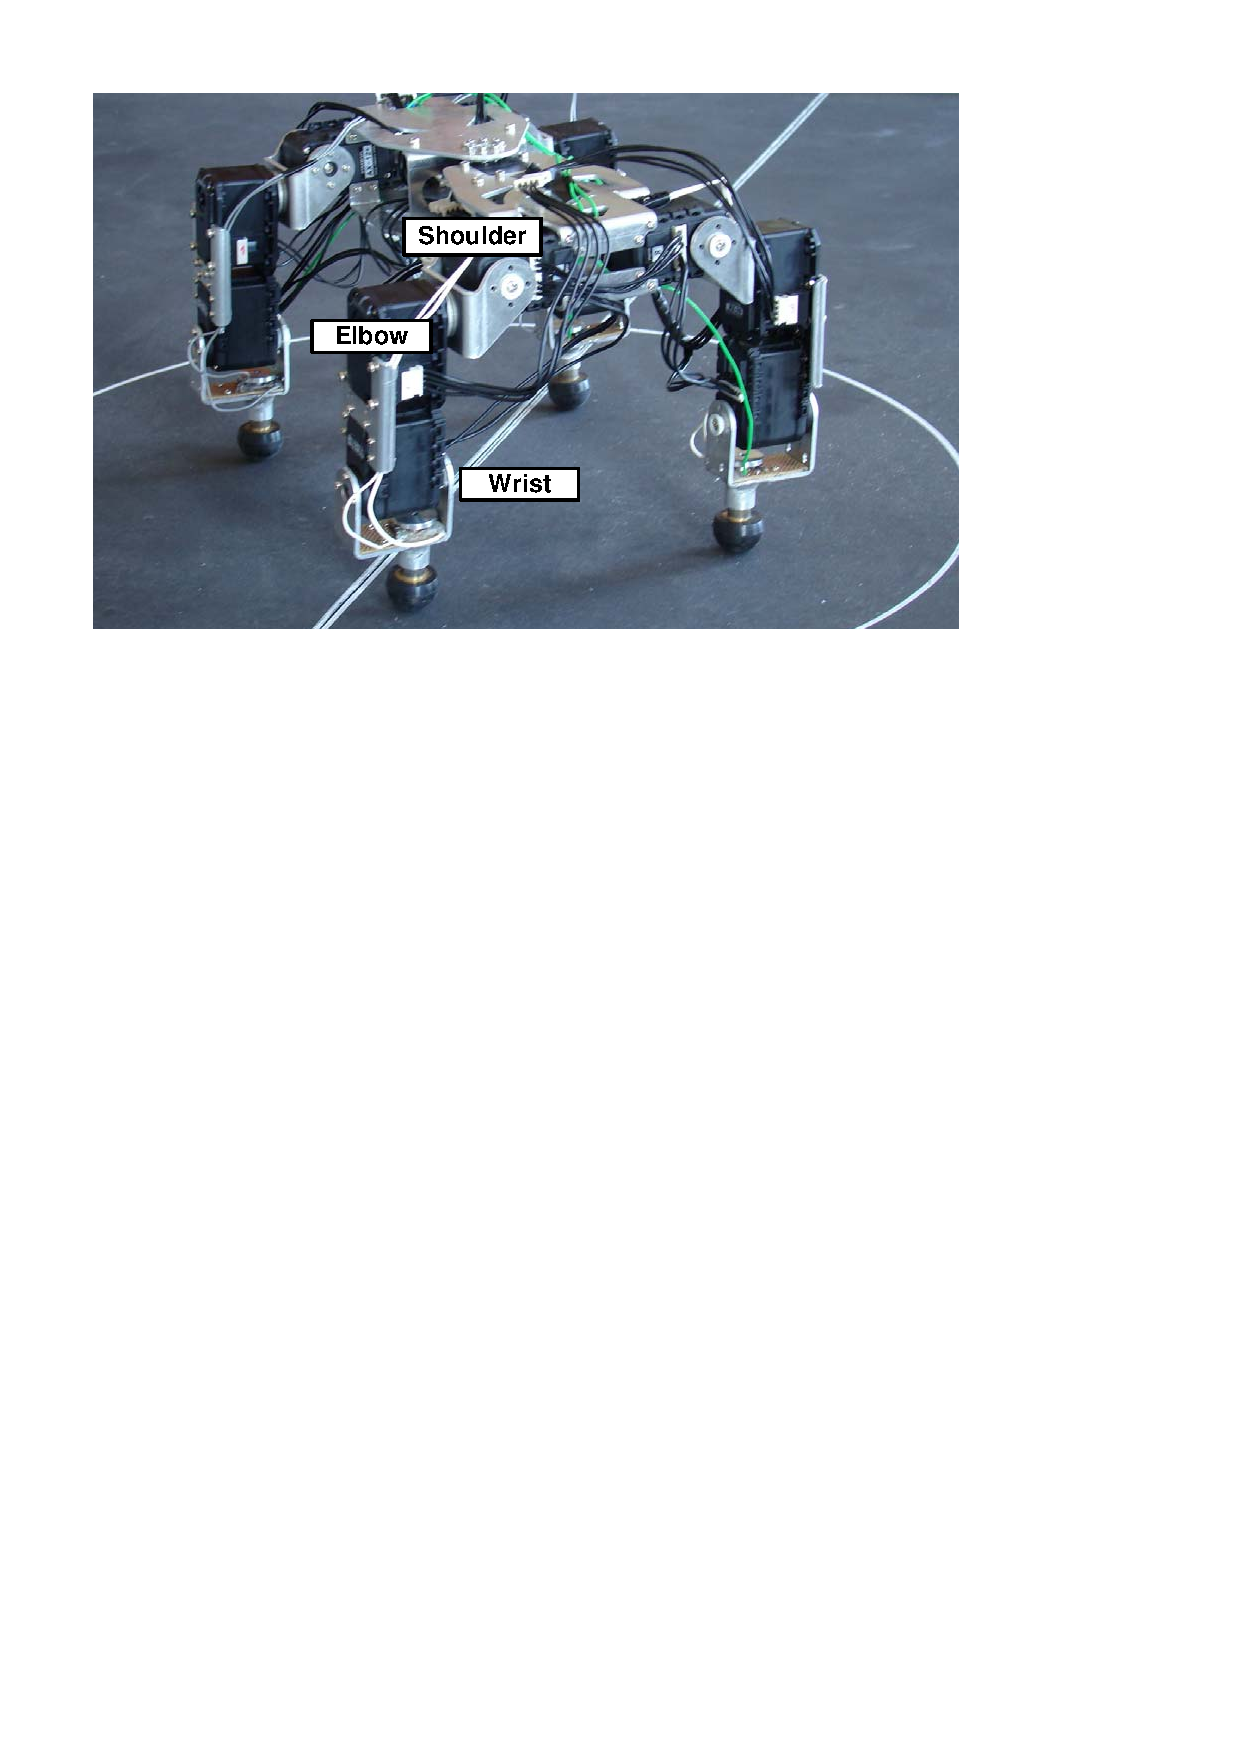
\includegraphics[width=85mm]{./pictures/Dynarobin_introduction_image.pdf}
                \caption{A quadruped robot}
                \label{fig:Dynarobin}
\end{figure}
 
Inspired by the agility of human and animal locomotion, over the last few decades  the number of research groups presented numerous robot leg designs, and the associated modeling and control \cite{CambridgeJournals:1345088}. The predominant method for the modeling of quadruped locomotion gaits like walking, running, trotting, and bouncing is a spring-mass model\cite{Blickhan01}. This paper postulates that a single leg, hopping locomotion can also be described with a spring-mass model. In order to obtain a compliant robot leg behavior, impedance control is used to emulate a virtual spring-mass system \cite{Havoutis01}. By attaching four legs to one central body complex dynamic problems arise. In order to provide a stable quadruped hopping sequence a lot of parameters needs to be observed: mass distribution, active and passive leg stiffness, ground stiffness, etc. This paper investigates how to improve locomotion stability of a dynamical system composed of four spring-masses by using a tail-like inertial appendage.
 
In Section \ref{sec:MathModel} a mathematical model of a quadruped robot (Fig. \ref{fig:Dynarobin}) together with a kinematic and a dynamic model of the tail is introduced. A single leg dynamics is modeled to mimic the behavior of an active spring-mass system. Building upon the results from Section \ref{sec:MathModel}, a recursive balancing algorithm is introduced in Section \ref{sec:Algorithm}. The algorithm is tested in the simulation environment which is described in Section \ref{sec:simulation}, along with the simulation results.




% Some research uses advanced variable stiffnes leg design %\cite{Hurst_2004_4785}\cite{Galloway}\cite{Jun:2009:DSV:1703775.1704089} which allows robot to run over a large variety %of terrains while adjusting their leg stiffness. All this research suggests that quadrupedal robot can be dynamically 5modeled as mass supported on four spring legs as shown in fig. 


